\section{Data Collection}
\label{ch:measurement}
Measuring the voice comparison involves three questions: whether participants perceived the self-similar voice as resembling their own, whether voice condition changed search performance, and how participants experienced the assistance. Answering them requires outcome measures together with an account of the speech each participant actually heard. This section therefore links voice identity, delivered speech, search events, and questionnaire responses, so that perceived similarity can be reported as a manipulation check and kept distinct from performance and experience outcomes. Detailed gaze and timing records support interpretation of these outcomes, and Appendix~\ref{app:instruments} retains instrument wording and scoring.


\subsection{Frame-Level Records and the Trial CSV}
The recording separates time-varying observations from trial summaries. Frame records retain application time, gaze origin and direction with tracking validity, head pose, available controller poses and input state, and the gaze/controller object-intersection evidence used by guidance. Object identities and transforms provide the scene needed for reconstruction; guidance transitions, agent decisions, actual speech playback, trigger selections, and pauses are recorded as events. A rendered frame can reuse a sensor observation, so frame count must not be reported as the number of independent eye-tracking samples.

For new rotational-search recordings, the trial replay snapshot additionally stores the wall bottom in recording-local coordinates, the wall height in metres, and a flag indicating that these bounds are available. Trial Review uses those recorded bounds to reconstruct the shorter walls. Earlier recordings without explicit bounds retain object-derived wall estimates and their original object positions; they are not rescaled to the current layout. These replay fields supplement the layout version and saved transforms and are distinct from the columns in the trial CSV. Analyses that include recordings from both layouts must retain that provenance rather than treat the geometry as unchanged.

Trial Review generates an Excel-compatible trial CSV with one row per trial. Its fields describe task performance, geometry, guidance exposure, and associated subjective responses (Table~\ref{tab:trial-fields}). Outcome, practice, provenance, and quality information accompany the exported records to support analysis and eligibility checks.

\begin{table}[htbp]\centering
\caption[Trial CSV contents]{Contents of the trial CSV. Unavailable values remain blank; reserved fields do not imply that a measure has been collected.}
\label{tab:trial-fields}
\small\tagpdfsetup{table/header-rows={1}}
\begin{tabularx}{\linewidth}{@{}p{0.23\linewidth}X@{}}\toprule
Group & Recorded or derived columns \\\midrule
Identity & Participant ID, trial ID, block index, voice condition. \\
Geometry & Absolute and signed nominal theta; actual signed head-to-target yaw; target-minus-head height; target distance. \\
Guidance and duration & Instruction count and search exposure in seconds. \\
Target contact & Time to first and final target gaze contact; first right-controller target contact; final selection. \\
Subjective context & NASA-TLX score; reserved subjective performance rating, currently blank pending an agreed instrument mapping. \\\bottomrule
\end{tabularx}
\end{table}

The export's post-onset head-relative yaw and height must not be relabeled as the proposed pre-cue cross-relative geometry. Gaze-contact times describe ray intersections, not validated fixations. A block-referenced questionnaire score may appear on multiple trial rows for convenience, but remains one block-level observation.

\subsection{From Interaction Events to Research Variables}
The recorded data serve two purposes: reconstructing what happened in a trial and estimating the study outcomes. Reconstruction requires observations and events at their original temporal resolution, whereas statistical analysis usually requires a more compact table. The project therefore keeps trial summaries separate from gaze, head/controller motion, object layouts, and event streams, treating each summary as a derived representation rather than a replacement for the underlying evidence.

Every derived value needs an identifiable source and a definition. A number called ``time to gaze'' is ambiguous unless it specifies the clock origin, the contact rule, validity handling, and the treatment of missing observations. The data contract preserves these meanings in separate fields.

Figure~\ref{fig:data-provenance} shows how a trial CSV remains linked to the underlying observations, so that values prepared for statistical analysis can still be traced to the records needed for trial reconstruction.

\begin{figure}[htbp]
\centering
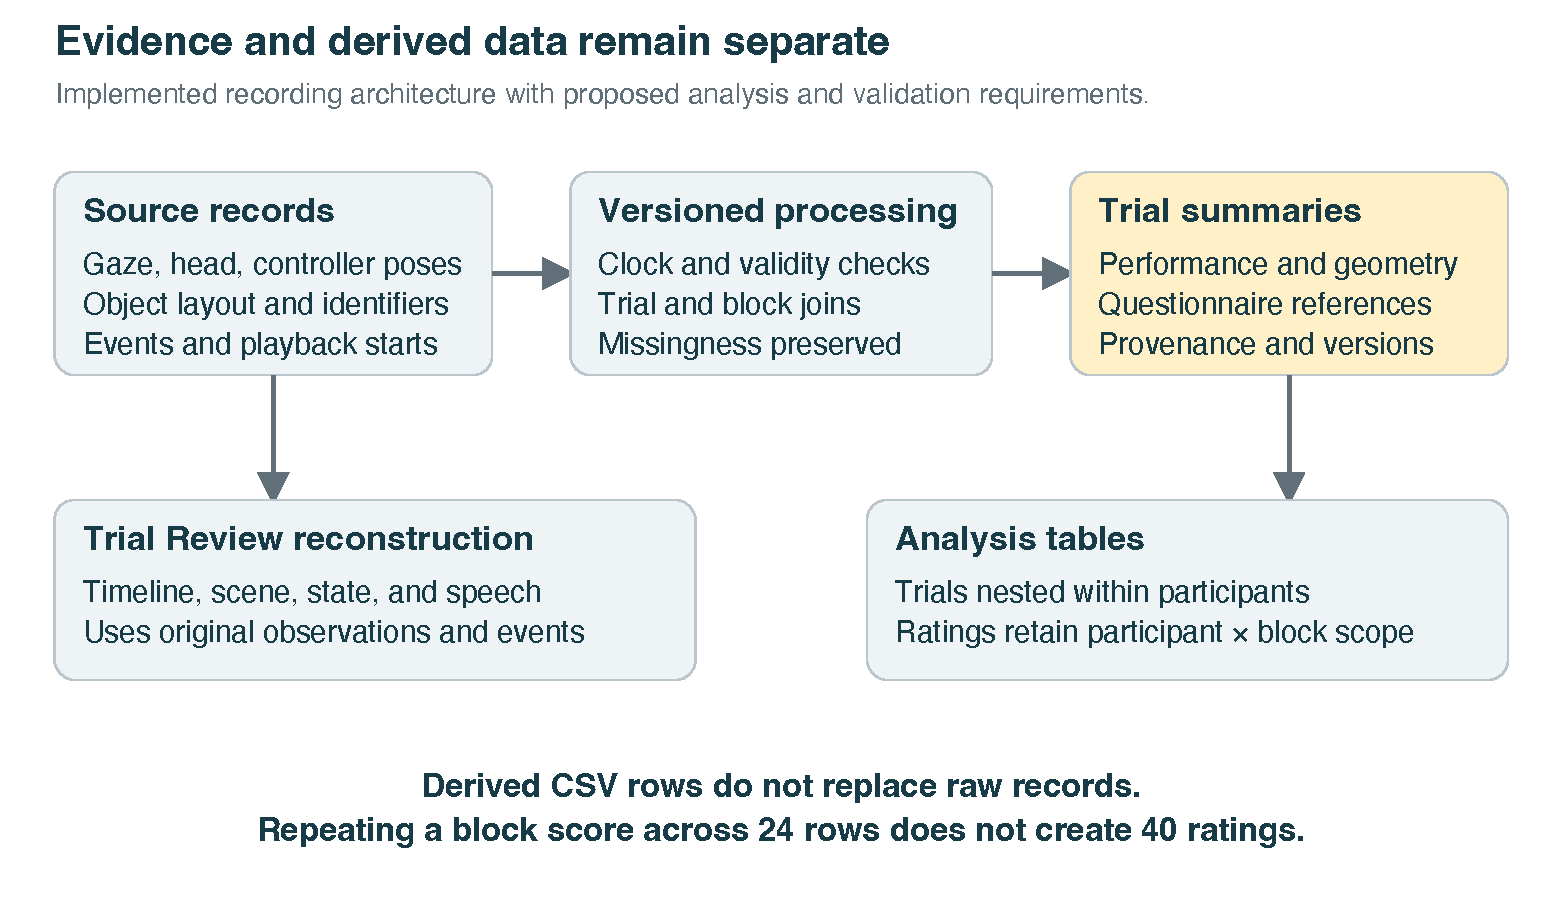
\includegraphics[width=\linewidth,alt={Raw observations and events feed versioned processing, trial summaries, Trial Review, and analysis tables.}]{figures/data-provenance.pdf}
\caption[Raw records, derived summaries, and analytical scope]{Recording and processing relationships. Source streams support reconstruction; derived summaries support analysis. Processing and scoring require versioned definitions. Repeating block-level ratings in trial rows does not create new independent observations.}
\label{fig:data-provenance}
\end{figure}


\subsection{Coordinate Frames and Starting Geometry}
Let $\mathbf{o}$ denote the saved trial reference origin, $\mathbf{c}$ the readiness-cross center, and $\mathbf{p}$ the target center. All three positions must be expressed in the same world coordinate frame. Let $\Pi(\mathbf{v})=(v_x,0,v_z)$ project a vector onto the horizontal plane. Define
\begin{equation}
\mathbf{a}=\Pi(\mathbf{c}-\mathbf{o}),\qquad
\mathbf{b}=\Pi(\mathbf{p}-\mathbf{o}).
\end{equation}
For nondegenerate vectors, the exact pre-cue starting angle is
\begin{equation}
\theta_0=\operatorname{atan2}\!\left(\hat{\mathbf{y}}\cdot(\mathbf{a}\times\mathbf{b}),\,\mathbf{a}\cdot\mathbf{b}\right)\frac{180}{\pi}.
\end{equation}
Verification compares the sign convention against Unity's world-up signed-angle convention using known left and right targets. The absolute value $|\theta_0|$ describes horizontal demand from the saved cross reference. Exactly backward targets require a documented tie convention, because $-180$ and $+180$ identify the same horizontal bearing, although the absolute magnitude remains 180 degrees in either case.

This calculation is a required addition to the frozen study data contract. The October 20, 2026 implementation alignment audit found that existing signed and absolute theta fields represented nominal wall geometry relative to the previous target wall. They must not be renamed or silently interpreted as exact pre-cue measurements. A new snapshot must save origin, cross, target, timestamp, frame, and coordinate-frame identifier before the opening cue. If a horizontal vector is degenerate, the angle is unavailable; substituting zero would falsely describe an easy starting configuration.

Nominal categories remain useful for allocation: each block contains eight scheduled trials in each absolute category, $0,45,90,135,180$ degrees. Because an object can be positioned away from the center of its assigned wall, however, its exact bearing need not equal the nominal category, and balance across categories therefore does not prove exact geometric matching between voice blocks. Both assigned and realized geometry are inspected.

The signed height difference is
\begin{equation}
\Delta h=p_y-c_y.
\end{equation}
Positive values identify targets above the cross center and negative values identify targets below it; this reference is not interchangeable with seated eye height. The planned 20-above/20-below allocation must be checked against realized positions and a prespecified near-zero rule, because the height scattering in the source snapshot did not enforce that balance.

The three-dimensional distance measure relies on a different observation: the first valid tracked head position $\mathbf{h}_k$ after reveal. Its value is $d=\|\mathbf{p}-\mathbf{h}_k\|_2$, in metres, and the timestamp of $\mathbf{h}_k$ must accompany the distance. Because this post-reveal measurement describes geometry at an observed head pose, it cannot recover an unrecorded pre-cue snapshot.

Figures~\ref{fig:starting-geometry} and~\ref{fig:height-reference} illustrate the proposed geometric contract using conceptual rather than recorded layouts.

\begin{figure}[htbp]
\centering
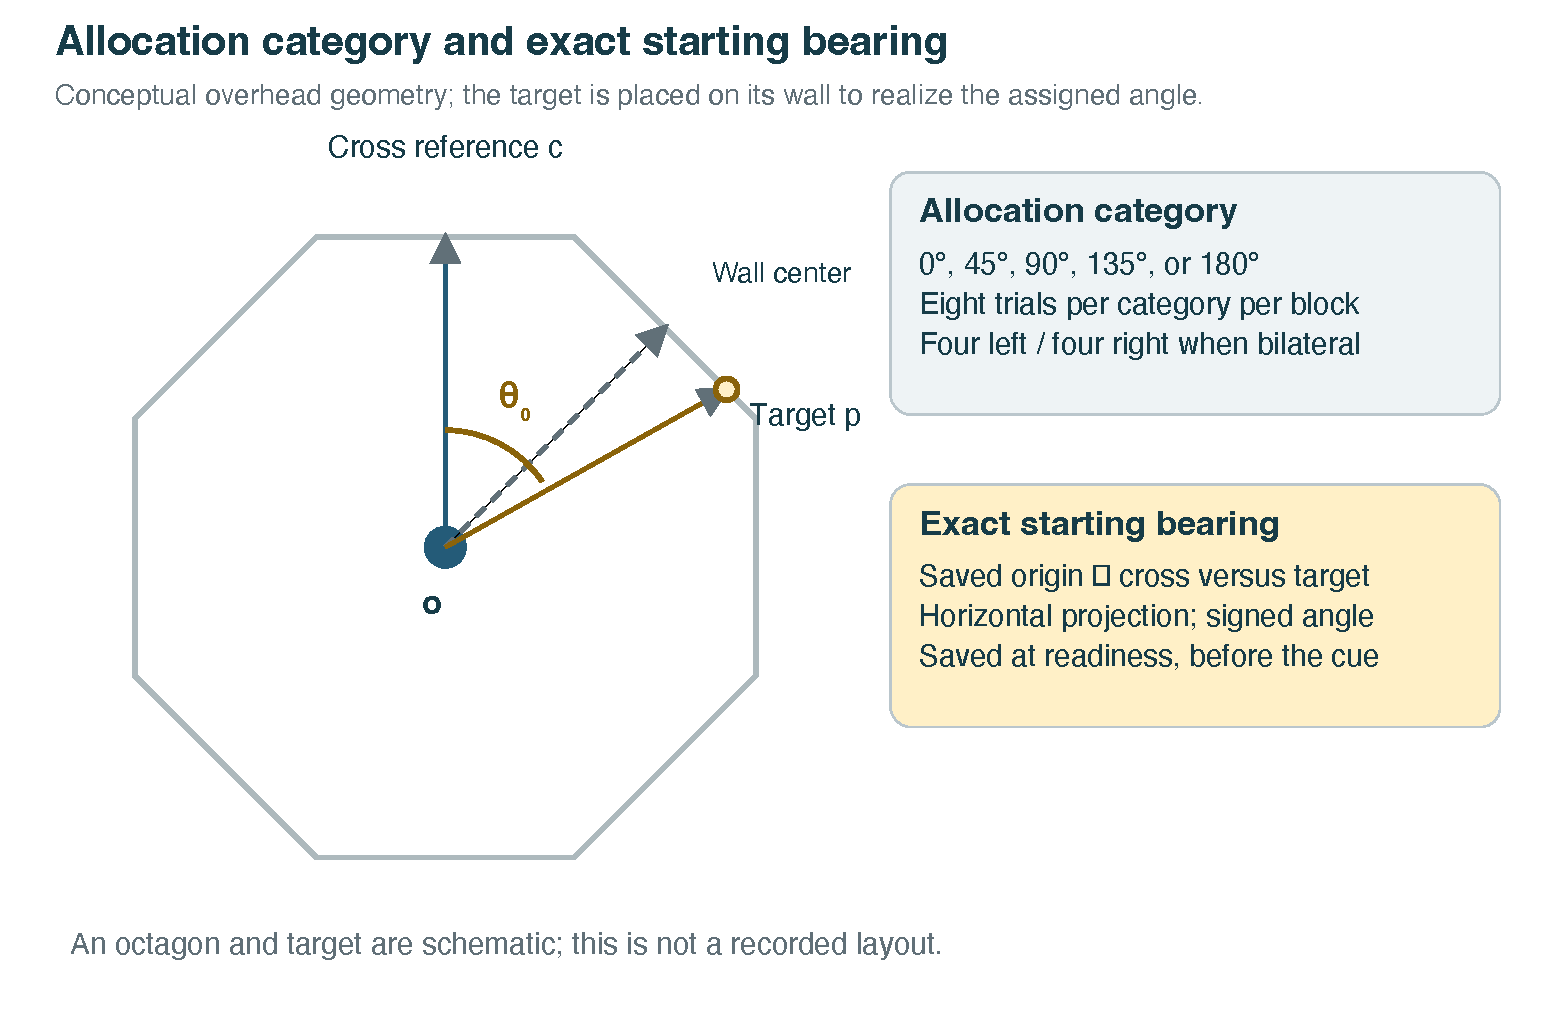
\includegraphics[width=\linewidth,alt={Overhead octagonal layout with origin, cross reference, nominal wall center, and an offset target showing distinct bearings.}]{figures/starting-geometry.pdf}
\caption[Nominal wall assignment and exact starting angle]{Conceptual overhead geometry. The target can be offset from its wall center, so an allocation category need not equal the realized starting bearing. The exact pre-cue snapshot remains an implementation requirement at the aligned checkpoint.}
\label{fig:starting-geometry}
\end{figure}


\begin{figure}[htbp]
\centering
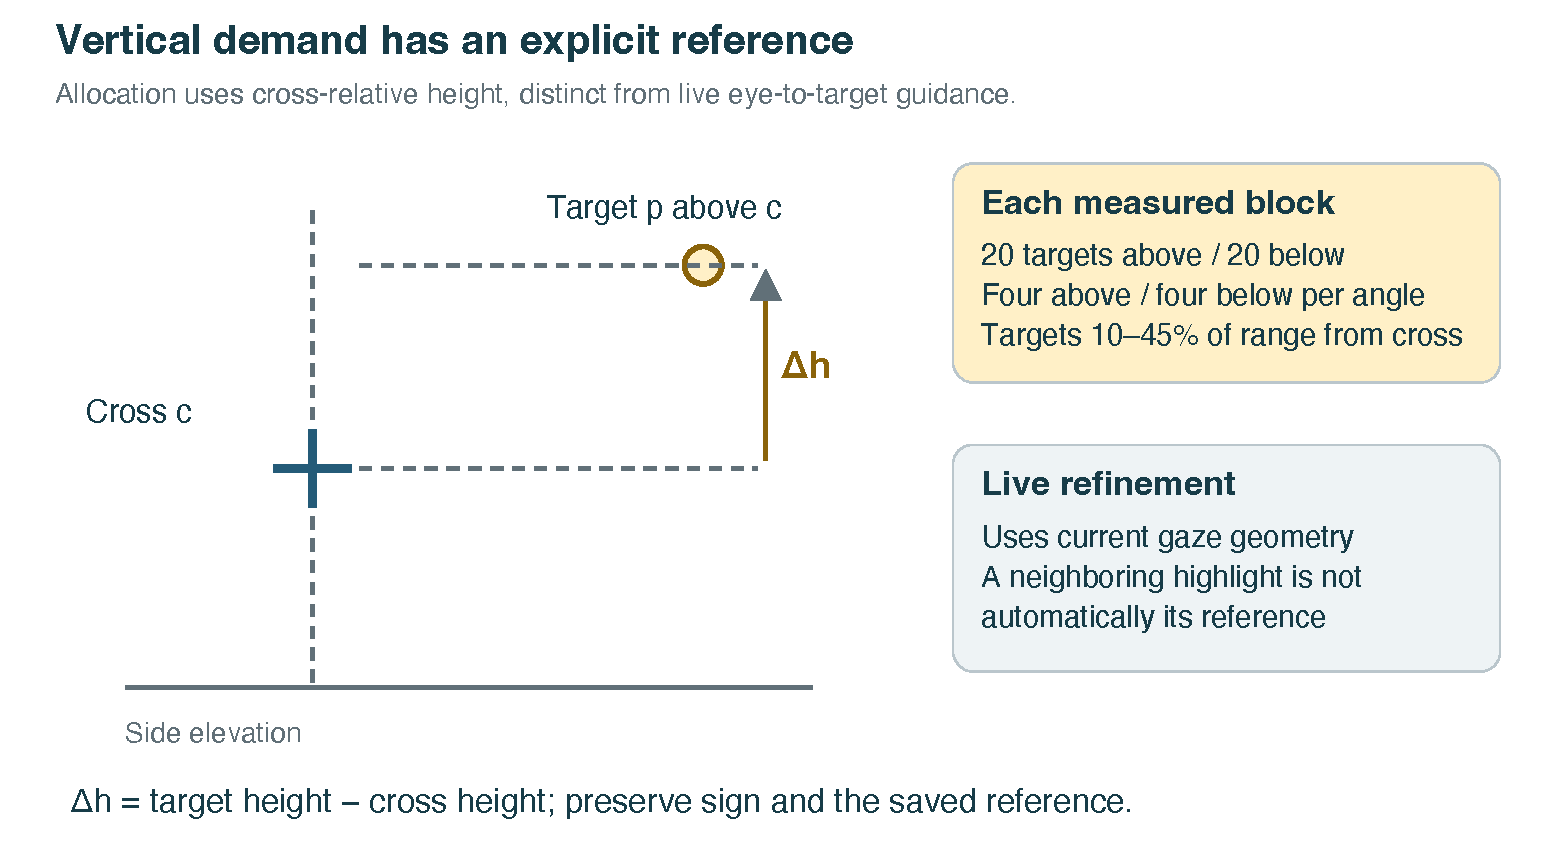
\includegraphics[width=\linewidth,alt={Side elevation of cross and target with positive signed height difference and a distinction between allocation and live refinement.}]{figures/height-reference.pdf}
\caption[Cross-relative height and live gaze refinement]{Conceptual side elevation for the proposed signed height difference. The target shown above the cross has positive height delta. The planned above/below quota and near-zero rule remain unresolved implementation and protocol checks; live vertical guidance uses current gaze geometry.}
\label{fig:height-reference}
\end{figure}


\subsection{Trial Clocks and Pause Intervals}
Let $t_r$ be object reveal, $t_s$ correct selection, and $\mathcal{P}$ the union of valid pause intervals. Active completion time is
\begin{equation}
T_{\mathrm{active}}=(t_s-t_r)-\mu\!\left([t_r,t_s]\cap\mathcal{P}\right),
\end{equation}
where $\mu$ denotes elapsed duration. Using the union prevents overlapping pause reasons, such as an application-focus pause that coincides with a researcher-requested pause, from being subtracted twice. The active clock remains stopped until every relevant pause reason has been resolved.

Readiness and opening speech precede reveal and are deliberately excluded from active search time. The measurement specification also includes the broader interval from opening-cue onset to selection. This measure includes the opening instruction, whose duration may differ across voices, while active completion time remains the primary outcome.

A stopped or timed-out trial has an observed duration and an outcome reason, but it does not have a successful completion time, and the analysis must not copy its stop timestamp into a success field. In the October 23 deadline implementation, a timeout records 25 seconds of active search exposure, a distinct timeout event, and an unsuccessful outcome. Software observes expiry on an update, while the exposure clock is capped at the deadline; event timestamps retain the actual observation time. Earlier development recordings retain their original durations and must not be retrospectively truncated to this limit. Source and receipt timestamps are likewise kept distinct, because a file that arrives late in the viewer reflects a transfer delay rather than necessarily a delay in the headset event.

Madritsch et al. distinguish overall task-completion time from active working time in an assistant-supported procedural task~\cite{madritsch2026assistance}, and their active measure is not assumed to correspond to the present clock. In Follow My Voice, active completion time includes ordinary waits for guidance between object reveal and correct selection, and only recorded pauses are excluded. Separate decision and playback timestamps help explain delivery delays without removing their task-level consequences from the primary outcome.

\subsection{Missed Targets}
A missed target is a search that reaches its recorded 25-second active-search deadline without a correct trigger selection. An incorrect selection followed by a correct selection before expiry is a completed search, with its selection error retained separately. Technical stops, withdrawal, and recordings without a known terminal outcome are not automatically classified as misses. For each participant, block, voice condition, and recorded deadline, the descriptive missed-target percentage is
\begin{equation}
M=100\frac{N_{\mathrm{timeout}}}{N_{\mathrm{selected}}+N_{\mathrm{timeout}}}.
\end{equation}
The denominator excludes practice and unresolved or technically interrupted attempts; their counts are reported alongside the percentage. A zero denominator yields an unavailable percentage. The full trial export implements \texttt{missed\_target} as 1 for timeout, 0 for successful completion, and blank otherwise. A separate \texttt{missed\_targets.csv} records grouped counts, deadlines, and development-data exclusion labels. Legacy records without an explicit deadline are retained but excluded from this deadline-specific percentage.

This outcome follows Chiossi et al.'s distinction between successful search and searches ending without selection~\cite{chiossi2024searching}. Their five-second task and the present 25-second, verbally guided task differ; percentages are therefore interpretable within each protocol and are not directly comparable benchmarks. The six unfinished searches in the earlier development recordings remain unfinished records, not retrospectively assigned missed targets.

\subsection{Eye-Event and Pupil Measures}
An implemented offline analysis preserves per-eye directions and pupil diameters from the HTC query stream, deduplicates repeated query timestamps, and separates search from readiness and pauses. Query receipts establish when software obtained data, not the sensor capture time or the independence of consecutive observations. Changes in trial or device, invalid tracking, reversed timestamps, and query gaps longer than 25 ms break continuity. Invalid per-eye observations and observed eye closure exclude nearby 200-ms intervals.

The fixation detector uses elapsed-time dispersion: the sum of horizontal and vertical angular ranges must remain within 1.8 degrees for at least 83 ms. This starting configuration follows the I-DT parameters reported by Chiossi et al.~\cite{chiossi2024searching}, within the detector family described by Salvucci and Goldberg~\cite{salvucci2000fixations}. Azimuth is unwrapped across the signed-angle boundary. The implementation retains event intervals and the duration of eligible segments; its counts are candidate classifications rather than validated fixations.

The saccade detector operates separately on eye-in-head angular velocity, with a provisional 60-degree-per-second threshold, a duration of 20--100 ms, at least two sampled intervals, and observed lower-velocity samples on either side. Intervals with head speed above 20 degrees per second or unavailable head pose are excluded. The reported rate divides event count by retained low-head-speed duration. It therefore describes a restricted observation window, not all saccades during search. These restrictions reduce head-turn ambiguity but do not validate event identity or establish sensor-level eye--head synchronization.

The Index of Pupillary Activity (IPA) calculation follows the wavelet-based approach of Duchowski et al.~\cite{duchowski2018ipa}. Each eye is processed separately. Accepted pupil segments contain valid finite diameters, last at least two seconds, meet a median query-rate screen of 60 Hz, and pass an interval-regularity screen. Within each accepted segment, values are resampled at its median query interval; no interpolation crosses rejected gaps or invalid observations. Level-two sym16 wavelet detail coefficients yield thresholded modulus maxima, which are counted per retained second. The implementation records its thresholds, resampling, numerical tolerance, and nearest-neighbor boundary convention. IPA is unavailable when no segment qualifies; it is never filled with zero to represent missing measurements.

Computational tests verify event boundaries, query deduplication, invalid-data handling, head-turn suppression, and wavelet calculations. They do not establish physiological validity. Independent event annotations, calibration checks, timing assessment, and held-out threshold evaluation remain necessary before fixation counts or saccade rates enter the participant analysis. Pupil-based interpretation additionally requires checks for luminance, gaze angle, blink artifacts, segment boundaries, and task-related confounds. IPA remains exploratory alongside NASA-TLX, rather than a validated estimate of workload in this apparatus. Final fixation duration on the target also remains unavailable until validated eye events can be joined to target areas of interest; the last ray contact is not a substitute.

\subsection{Gaze Contact, Vicinity, Pointing, and Selection}
Four event families are central to interpretation: a valid eye ray can intersect the target collider; a gaze direction can satisfy the larger target-vicinity rule; the right-controller ray can intersect the target; and a trigger press can select the target. These events can occur at different times and need not occur in that order in every recorded sample sequence.

The first gaze-contact latency uses the first valid recorded target-ray intersection after reveal. The last gaze-contact time uses the last such intersection before trial end. Neither is a fixation duration. If no contact is observed because of a blink, acquisition gap, or a path that only enters the broader vicinity, the contact field remains missing.

Vicinity qualification is an interaction rule rather than a fixation classifier. In the documented system, a target can be acknowledged after 100 ms of valid qualifying evidence, with overlapping regions resolved to a single closest candidate. The rule trades exact collider intersection for a tolerance intended to make feedback usable, but an overly large region can produce premature acknowledgment even when the timing gate behaves correctly. The tolerance must therefore be logged and piloted; its study-release value has not been frozen, and the default ring in the synthetic viewer screenshot is not a validated study setting.

Controller pointing is a distinct input observation, but its spoken acknowledgment is not independent of gaze: the documented rule requires a qualified one-second controller hold with valid gaze in the target vicinity when the speech scheduler permits the acknowledgment to play. Before the hold completes, a valid target hit already suppresses contradictory away-directions; this suppression prevents a direction such as ``go back down'' from being delivered while the controller is already on the target, without announcing that the hold has qualified. Correct trigger selection is the only event that successfully completes the search; a stop or timeout has a different outcome.

Figure~\ref{fig:evidence-events} contrasts the two acknowledgment events with trial completion.

\begin{figure}[htbp]
\centering
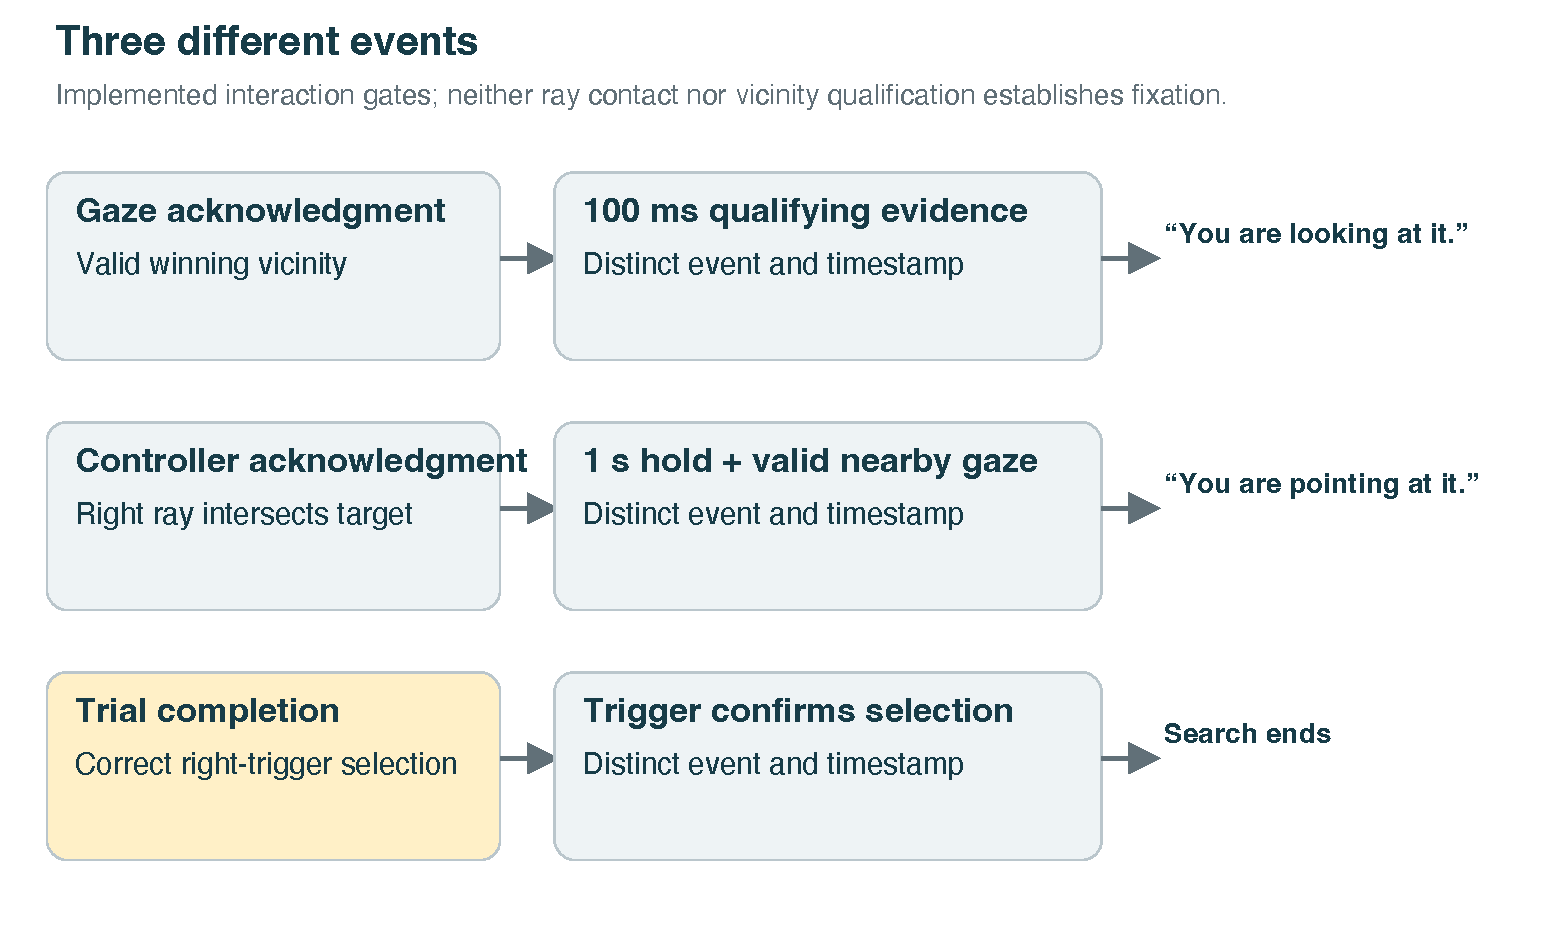
\includegraphics[width=\linewidth,alt={Three separate rows show qualified gaze, qualified controller pointing, and correct trigger selection as distinct events.}]{figures/evidence-events.pdf}
\caption[Gaze acknowledgment, pointing acknowledgment, and completion]{Implemented interaction distinctions. Gaze acknowledgment uses a 100-ms qualifying vicinity gate; pointing acknowledgment uses a one-second controller hold with required valid nearby gaze. A correct trigger selection completes the trial independently of whether either acknowledgment was spoken. These are interaction gates, not validated fixation measures.}
\label{fig:evidence-events}
\end{figure}


\subsection{Acquisition Rate, Validity, and Gaps}
A render loop can query an eye-tracking API frequently without receiving a new hardware observation each time, so the effective acquisition rate must be estimated from distinct source observations. If $n$ unique observations span source times $t_1$ through $t_n$, a basic rate summary is $(n-1)/(t_n-t_1)$. Because a mean alone can conceal bursty delivery, the distribution of successive intervals, repeated timestamps, invalid observations, and long gaps must accompany that average.

Application timestamps describe when data were handled, whereas source timestamps describe when the tracking observation was produced, if the API exposes them reliably. A clock-domain mapping must therefore be established before age or latency is computed across these clocks. If unique source timing is unavailable, the report states that limitation rather than infer 120-Hz binocular delivery from polling or headset specifications.

Spatial validation compares gaze direction with known independent targets. Angular error is computed from normalized gaze and expected target directions, with invalid observations excluded from the error distribution but retained in availability summaries. Precision and bias should be considered separately, since a stable offset and a noisy signal can produce different guidance failures even when their average angular error is similar. The validation procedure must also describe target exposure, head pose, corrective lenses, and headset adjustments.

\subsection{Motion, Coverage, and Instructions}
Gross translation sums Euclidean differences between adjacent valid head positions, and gross rotation sums shortest quaternion angular differences; invalid intervals, excessive gaps, and pauses break the accumulation. Gross movement is a total, not a rate. If a separate movement-rate outcome is derived, its denominator is observed covered time rather than the entire nominal session, because otherwise two runs with different data loss could produce misleadingly different movement rates.

Fixed-axis components derived from rotation vectors are not Euler yaw, pitch, and roll, and their labels retain the actual calculation. Head motion also does not directly measure swivel-chair rotation, because the head can move relative to the torso and chair.

Instruction counts use actual software playback starts; a requested cue, a rejected model answer, and a prefetched clip are not delivered instructions. Opening cues, search guidance, acknowledgments, reminders, and success speech have separate categories. The planned total of delivered active-search assistance includes directional guidance, gaze/pointing acknowledgments, and selection reminders, with each category also reported separately, while opening and success speech remain outside that total. Interrupted speech counts as started speech but retains its completion status, so it should not be treated as if the participant heard every word.

\subsection{Sequence-Level Latency}
For a qualified event, let $t_q$ denote the earliest supported qualification time and $t_p$ the actual software playback start of the corresponding acknowledgment. The primary engineering delay is
\begin{equation}
L_{\mathrm{software}}=t_p-t_q.
\end{equation}
This is not acoustic latency at the participant's ear, because audio-device buffering and the physical sound path require a separate measurement. Gaze and controller qualification times must also use their own definitions, since comparing a controller acknowledgment against first gaze contact would inflate or misattribute its delay.

Repeated requests about one continuously qualified event form a single episode, so a sequence can include several decisions by Jev to wait without creating several independent missed confirmations. An episode ends with playback, disqualification, trial termination, or a defined reset, and the evaluation reports how those endpoints were assigned, marking incomplete evidence as unknown.

Where logs support attribution, waiting is divided into model response, explicit model deferral, scheduling, existing speech, and audio readiness. Because these intervals may overlap, they are not summed unless they are represented as a nonoverlapping partition of the critical path. The full event timeline remains the authority when aggregate attribution is ambiguous.

Figure~\ref{fig:latency-definition} separates intentional evidence qualification from subsequent delivery delay.

\begin{figure}[htbp]
\centering
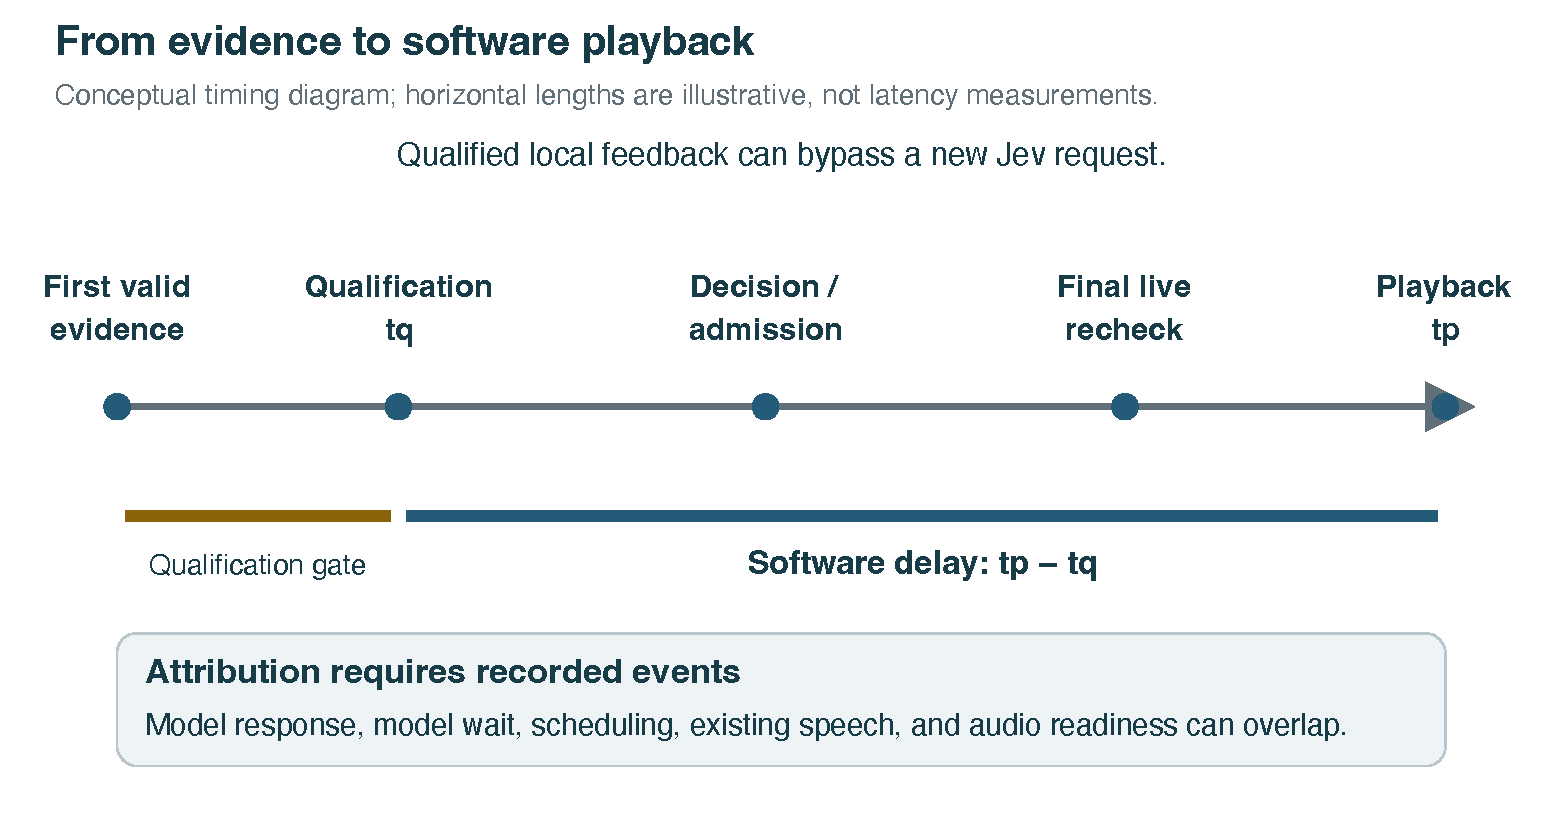
\includegraphics[width=\linewidth,alt={Timeline distinguishes first valid evidence, qualification, admission, final recheck, and software playback; intervals are illustrative.}]{figures/latency-definition.pdf}
\caption[Qualification-to-playback latency and its boundaries]{Conceptual event timeline, not a measured trace. Software delivery delay begins at supported qualification and ends at actual software playback start. The preceding qualification gate and the unmeasured acoustic path are separate quantities. Qualified local feedback can avoid a new cloud request.}
\label{fig:latency-definition}
\end{figure}



Table~\ref{tab:latency-contract} lists the principal timing variables with their endpoints and interpretive limits.
\begin{table}[htbp]
\centering
\caption[Timing variables and evidence boundaries]{Timing contract for planned analysis and engineering evaluation. All cross-clock comparisons require an established mapping; unavailable evidence is not assigned a zero duration.}
\label{tab:latency-contract}
\small
\tagpdfsetup{table/header-rows={1}}
\begin{tabularx}{\linewidth}{@{}p{0.23\linewidth}p{0.31\linewidth}X@{}}
\toprule
Quantity & Endpoints & Interpretation limit \\\midrule
Active completion & Reveal to correct trigger, less union of pauses & Excludes readiness and opening cue; unfinished trials remain unfinished. \\
First gaze contact & Reveal to first valid target-ray hit on active clock & Intersection, not fixation or vicinity acknowledgment. \\
First pointing contact & Reveal to first tracked right-ray hit on active clock & Not the one-second hold or trigger selection. \\
Jev response latency & Request dispatch to response receipt & A response can be deferred, canceled, or stale. \\
Confirmation delivery & Qualified evidence to matching actual software playback & Separate gaze and pointing episodes; not acoustic latency. \\
Live transfer lag & Source event to viewer receipt, if clocks are mapped & Describes transport, not headset decision delay. \\\bottomrule
\end{tabularx}
\end{table}

\subsection{Questionnaire Joins and Versioning}
Final questionnaire administration is separate from the block to which a response refers. A response collected after both blocks retains both its final-administration timing and a Block 1 or Block 2 reference, and the actual voice identifier must be joined through the saved order rather than inferred from block number. Practice is excluded from measured block outcomes even though it uses the first voice.

A convenience export may repeat a block-level workload score on every trial row, but this repetition does not create 40 independent workload observations. The analytical dataset identifies participant-by-block scope and collapses duplicate joins when estimating questionnaire effects. Raw responses, score direction, scale bounds, item identifiers, instrument version, and missingness remain available.

The current NASA-TLX adaptation uses 0--10 ratings, whereas older development exports used 0--100, so automatic scoring must require explicit range metadata. A separately named normalized score can support comparison, but raw values must remain unchanged, and legacy responses whose performance anchors are unknown cannot be scored by guessing their direction. Complete-subscale scoring for IMI and agent-perception measures requires verification before confirmatory analysis.
